\section{Dynamic hypothesis}
\subsection{Causal loop diagram}
Figure \ref{img:causalloop} shows the causal loop diagram for the model in study.
\begin{figure}[H]
	\centering
    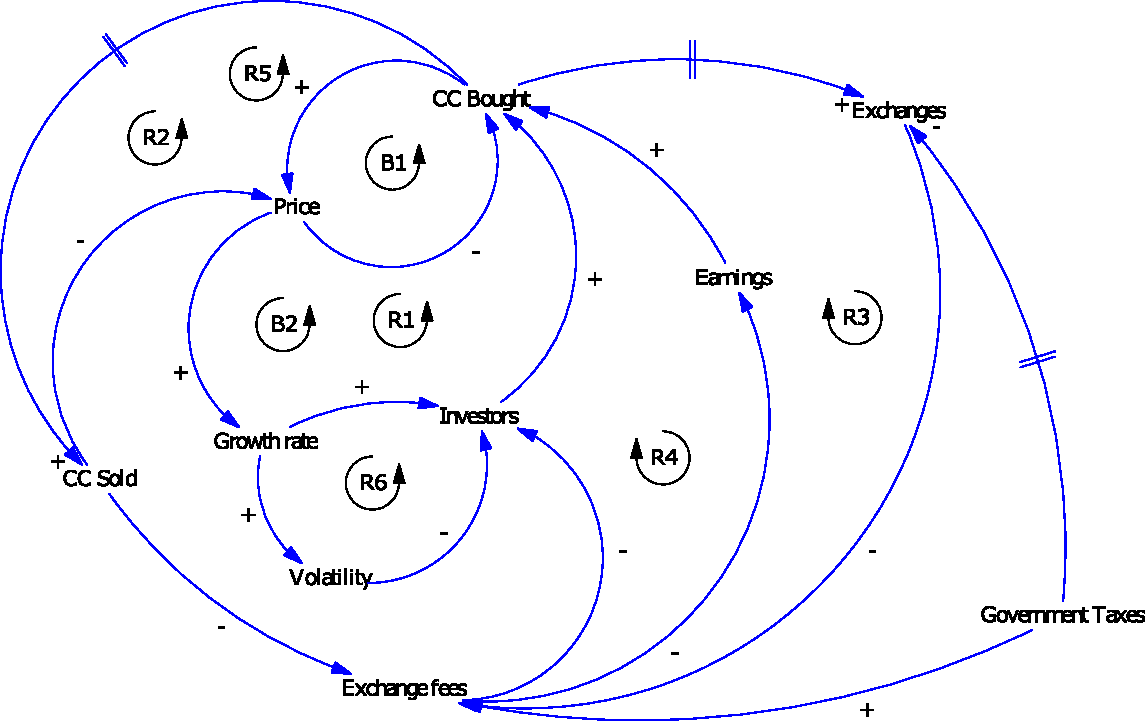
\includegraphics[scale=0.75]{files/CausalLoopDiagram.pdf}
    \caption{Causal loop diagram for cryptocurrency exchange market.}
    \label{img:causalloop}
\end{figure}

\subsection{Feedback loops}
\subsubsection{Reinforcing}
	\begin{itemize}
	\item \textit{R1 - Amount of CC bought due to investors:} This loop explains how the price increases due to the purchase of new CC; because the growth is defined as a change in a period of time, it is clear that it will increment as well. Now, as the CC is growing, more people will be interested in investing, which implies more CC bought. Shown in Figure \ref{R1}.
	\begin{figure}[H]
		\centering
        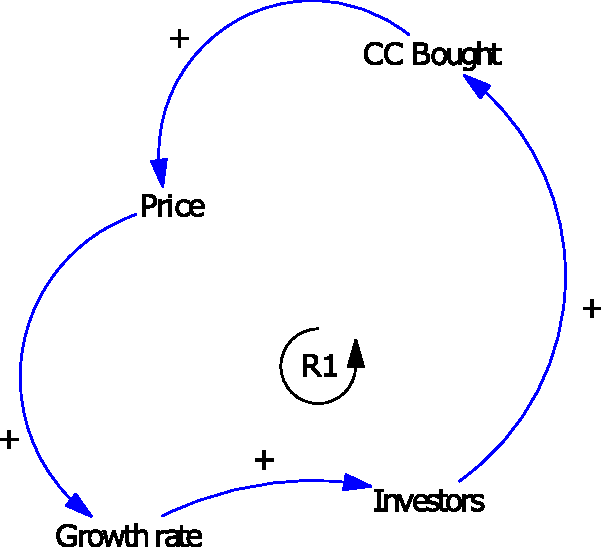
\includegraphics[scale=0.5]{files/R1.pdf}
        \caption{Loop R1.}
        \label{R1}
	\end{figure}
    \item \textit{R2 - Amount of CC bought due to earnings:} This reinforcing loop explains how exchange fees affect the amount of CC bought due to their earnings, which, in a future, will be sold; this implies a change on the exchange fees because the selling procedure is through a exchange house. Shown in Figure \ref{R2}.
    \begin{figure}[H]
		\centering
        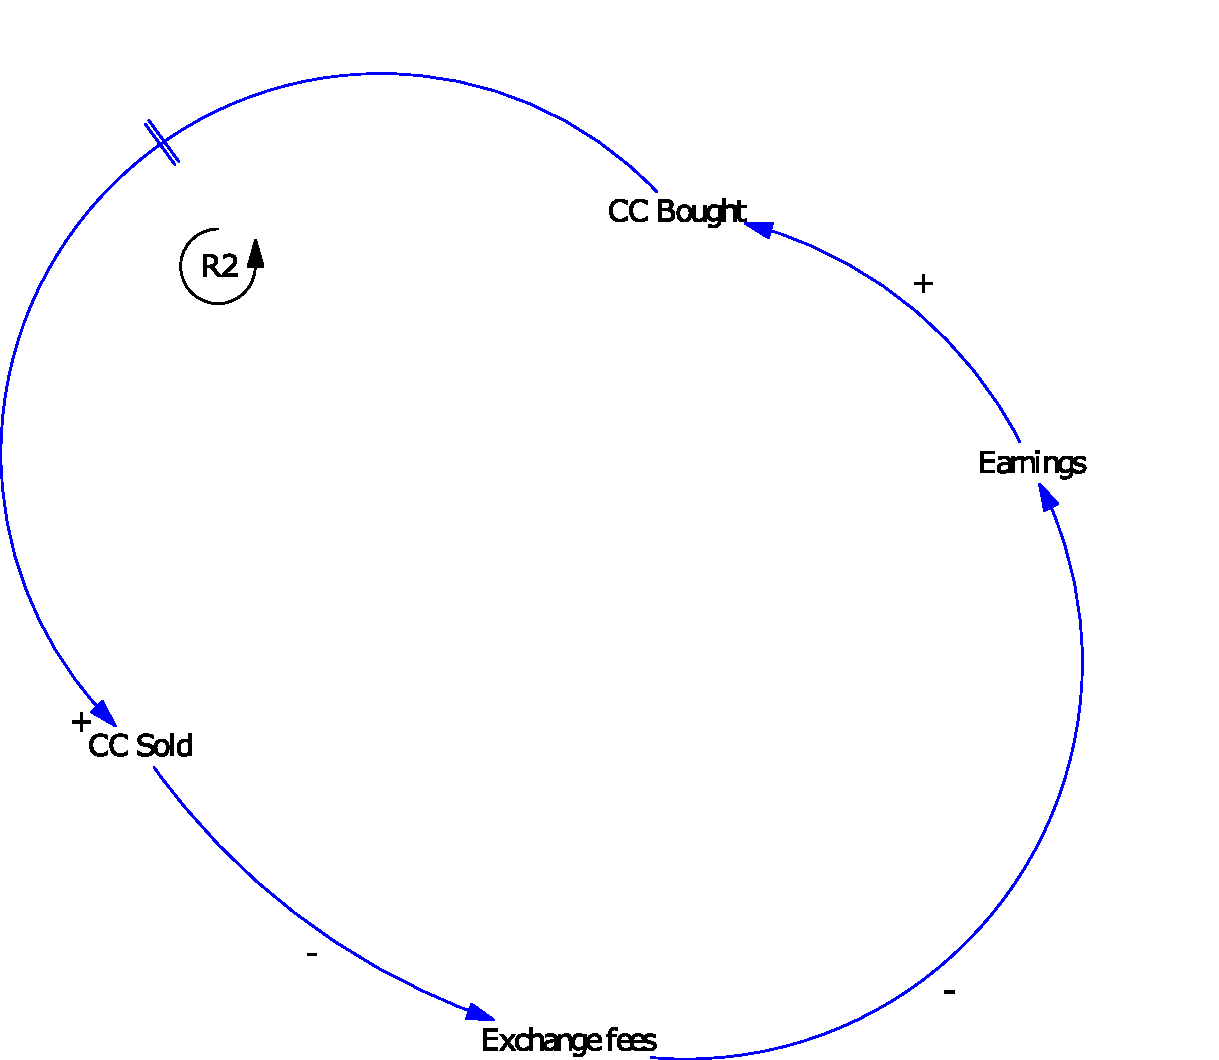
\includegraphics[scale=0.4]{files/R2.pdf}
        \caption{Loop R2.}
        \label{R2}
	\end{figure}
    \item \textit{R3 - Earnings due to exchange fees:} Let us imagine a market with a lot of exchanges, in order to compete with the other exchange houses, they will have to reduce their fees; therefore, people will obtain higher revenue. This encourages people to buy more CCs. Shown in Figure \ref{R3}.
    \begin{figure}[H]
		\centering
        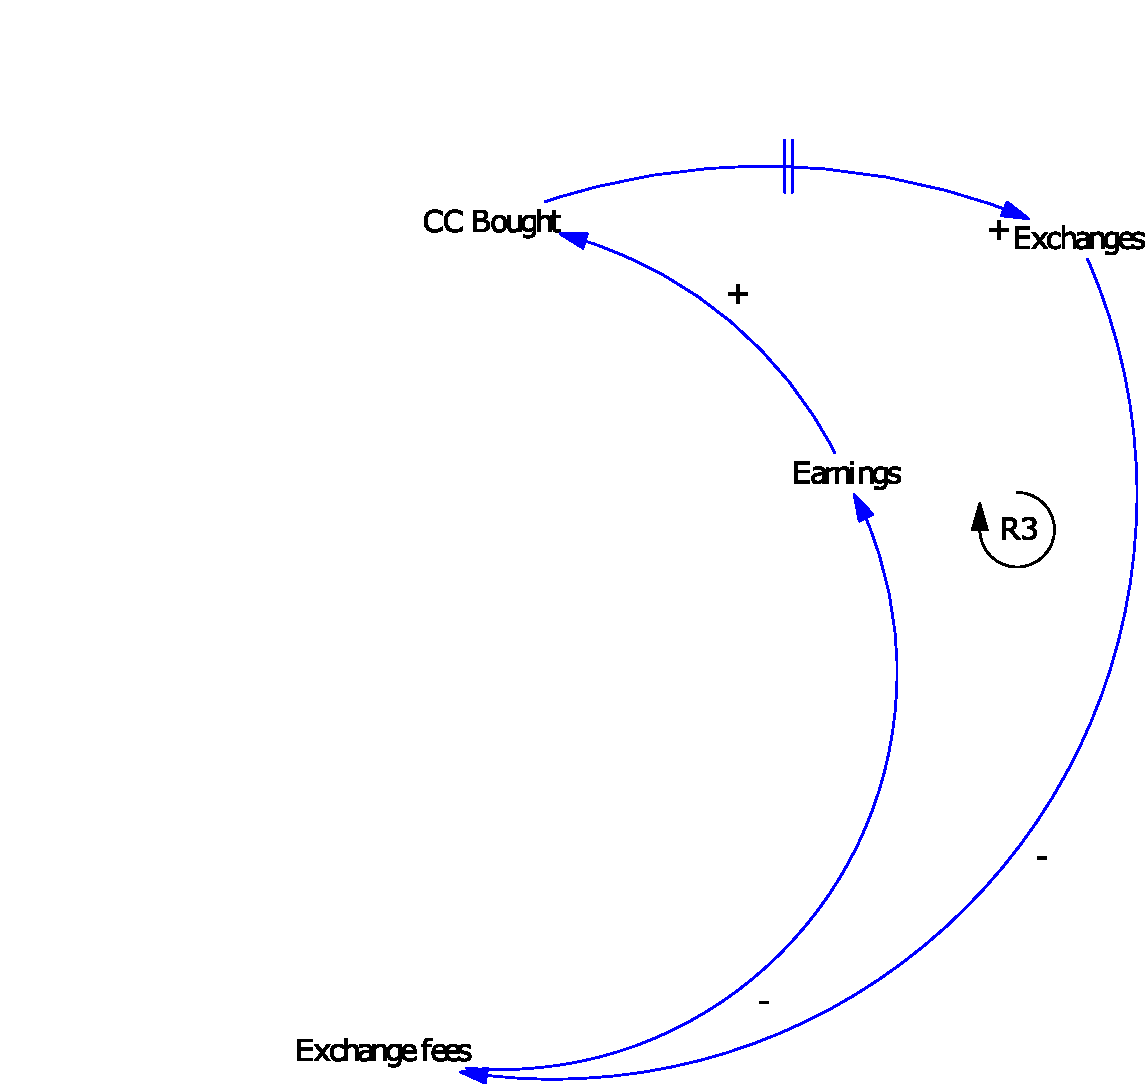
\includegraphics[scale=0.5]{files/R3.pdf}
        \caption{Loop R3.}
        \label{R3}
	\end{figure}
    \item \textit{R4 - Investors due to exchange fees:} This is similar to last loop, since the exchange fees determines the number of investors there will be; and they, as well, determine the number of CC bought. As we said, the number of CC bought influences the number of exchange houses and, due to market competition they will have to change their fees. Shown in Figure \ref{R4}.
    \begin{figure}[H]
		\centering
        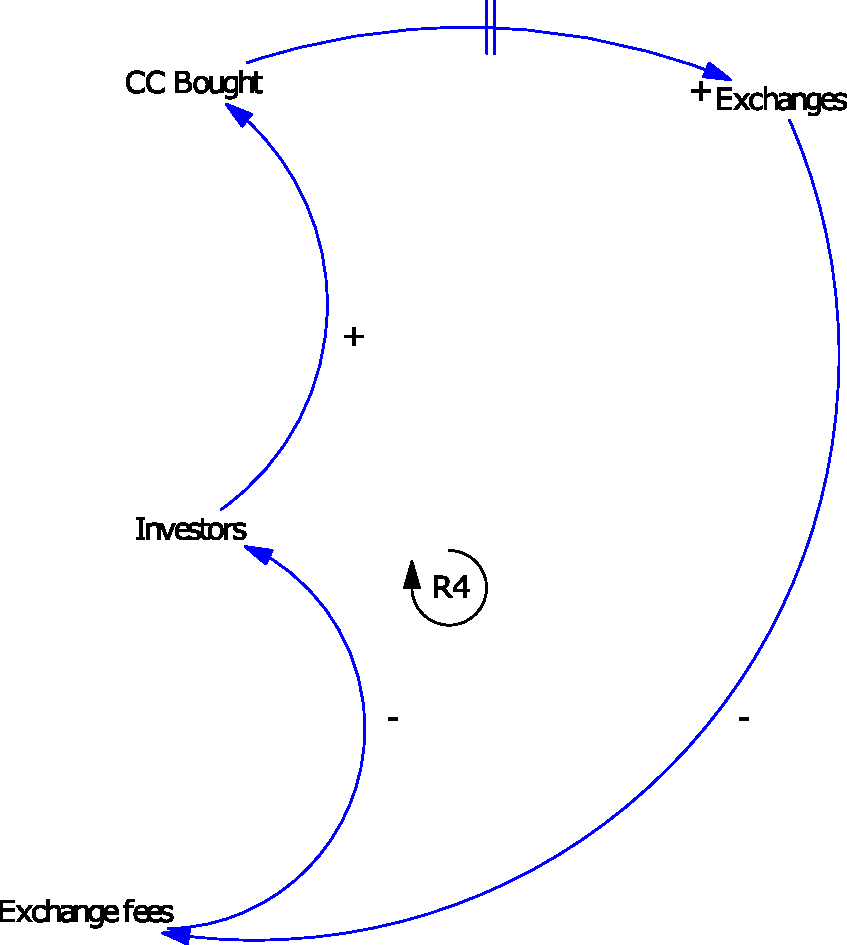
\includegraphics[scale=0.5]{files/R4.pdf}
        \caption{Loop R4.}
        \label{R4}
	\end{figure}
    \item \textit{R5 - Delay between purchase and sell of CCs:} The price defines both the amount of CC bought and sold; if, in the future, there are more CC bought, it will produce more sells. Shown in Figure \ref{R5}.
    \begin{figure}[H]
		\centering
        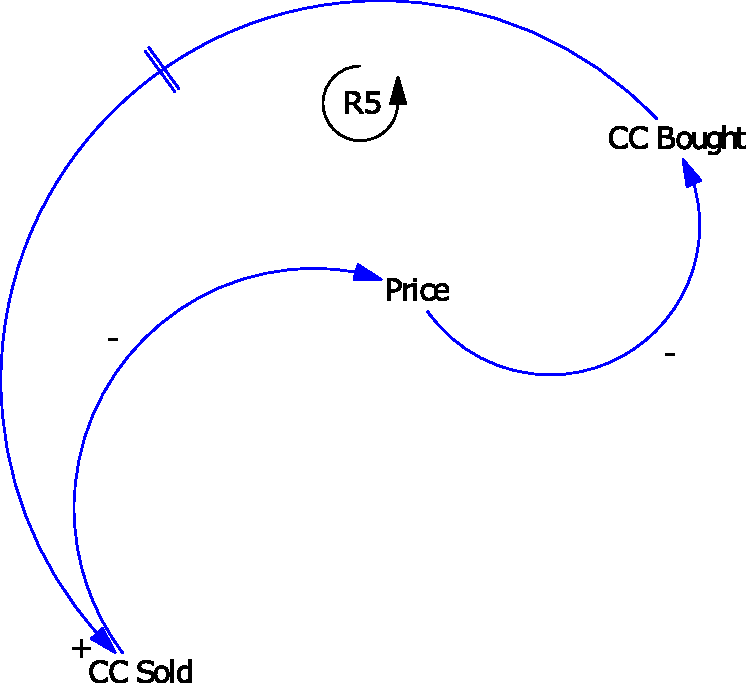
\includegraphics[scale=0.5]{files/R5.pdf}
        \caption{Loop R5.}
        \label{R5}
	\end{figure}
    \item \textit{R6 - Investing leads to more investors:} If we define the volatility as the risk of an investment, if there is more, there will be less investors and CC bought; therefore, there will not be an increment in the CC sold and the price will increase. Clearly, the growth rate will increase as well. Shown in Figure \ref{R6}.
    \begin{figure}[H]
		\centering
        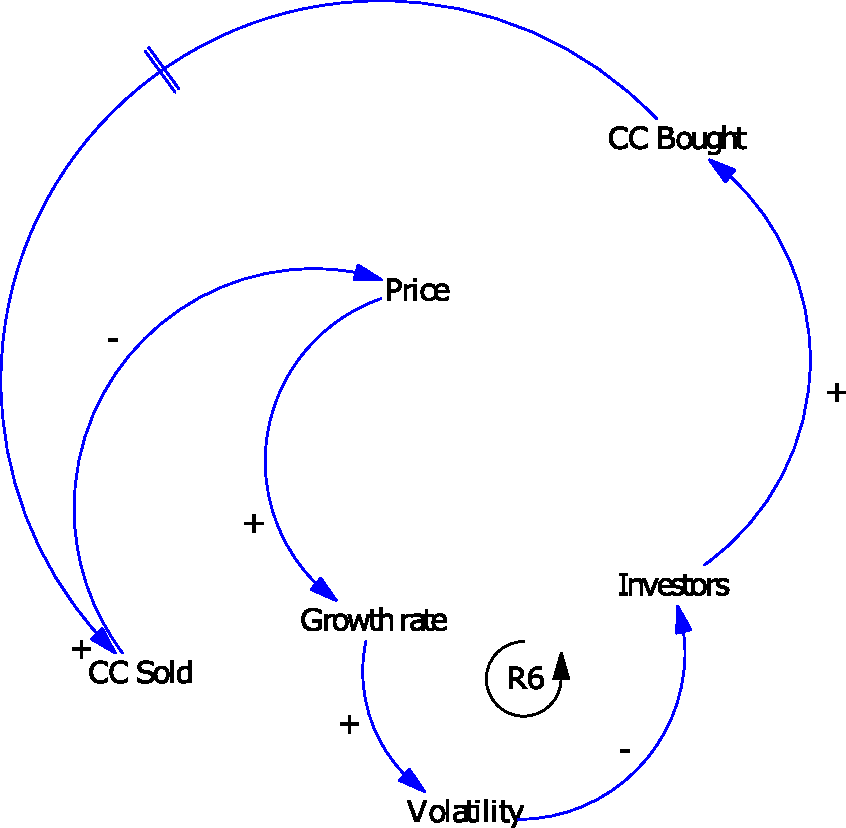
\includegraphics[scale=0.5]{files/R6.pdf}
        \caption{Loop R6.}
        \label{R6}
	\end{figure}
	\end{itemize}
\subsubsection{Balancing}
\begin{itemize}
	\item \textit{B1 - Balancing price:} If investors start buying more coins of a CC, then the price increments. On the other hand, when the price starts to go up, then people can't afford to buy as much CC as before so, naturally it reduces the number of CC bought by the public. Shown in Figure \ref{B1}.
	\begin{figure}[H]
		\centering
        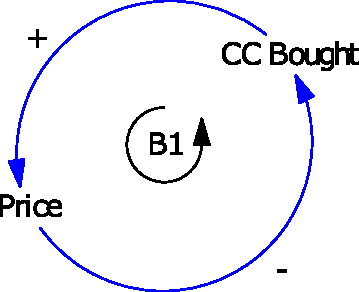
\includegraphics[scale=0.6]{files/B1.pdf}
        \caption{Loop B1.}
        \label{B1}
	\end{figure}
    
	\item \textit{B1 - Price due to Investors:} If the CC price starts growing faster, then more costumers will invest in that CC as it shows better profits. In this manner, a increase in investors will augment the number of CC bought. In a delay, investors who bought this coins will sell them which accordingly reduces the price. Finally, the growth rate reduces because of the decline of price. Shown in Figure \ref{B2}.
	\begin{figure}[H]
		\centering
        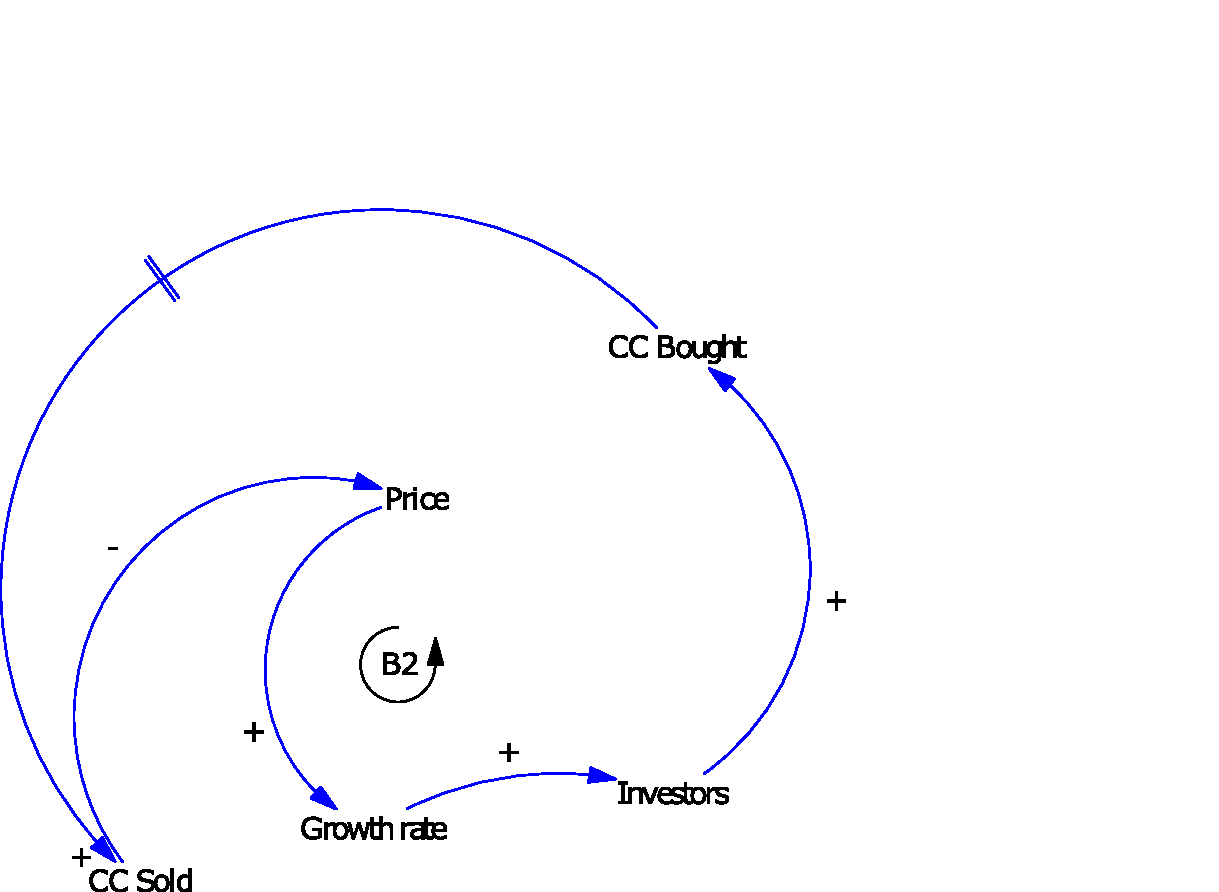
\includegraphics[scale=0.5]{files/B2.pdf}
        \caption{Loop B2.}
        \label{B2}
	\end{figure}
\end{itemize}




